\documentclass{article}

\usepackage{booktabs}
\usepackage{amsmath}
\usepackage{amssymb}
\usepackage{hyperref}
\usepackage{enumitem}
\usepackage[accepted]{dlaiml2025}
\usepackage{graphicx}
\usepackage{microtype}
\usepackage{xcolor}
\usepackage{float}

\graphicspath{{figures/}}

\dlaititlerunning{Attention Fingerprints of Adversarial Perturbations}


\begin{document}

\twocolumn[
  \dlaititle{Attention Fingerprints of Adversarial Perturbations \\
    in Flow-Matching Generative Models}

  \begin{center}October 2026\end{center}

  \begin{dlaiauthorlist}
    \dlaiauthor{Marco Galletti}{sapienza}
  \end{dlaiauthorlist}

  \dlaiaffiliation{sapienza}{Sapienza University of Rome}
  \dlaicorrespondingauthor{Marco Galletti}{galletti.2109043@studenti.uniroma1.it}

  \vskip 0.3in
]

\printAffiliationsAndNotice{\textit{Supervisor: Prof. Iacopo Masi}}

\begin{abstract}
We measure the fingerprint an adversarial perturbation of the initial noise leaves in the self-attention maps of a generative sampler and ask whether it differs between a UNet and a diffusion transformer. A UNet-B and a SiT-B/2 (the DiT-B/2 architecture trained with flow matching; we call it the DiT) are trained from scratch under one protocol and attacked with the same $L_\infty$ PGD on the initial noise through the 25-step sampler, on 500 shared seeds. The fingerprint is the drop in effective rank relative to a random control of equal budget; hypotheses, margins and controls were pre-registered. In both models the rank falls in the last sampling steps (effect size about 1.3) although the attack never observes the maps, and the FID of attacked samples decreases. The cross-model magnitude difference is detectable ($-0.006$) but within the pre-registered margin of 0.010 on the absolute scale; the localization difference is wide but cannot be attributed to the architecture, since a less converged DiT checkpoint differs comparably, and the registered reading is that it tracks convergence. Under the pre-registered rule the architectures are not distinguishable, one of the two outcomes the design was built to interpret. Exploratively, a late-window rank threshold detects attacked samples (AUC up to 0.99) and transfers across backbones, and the attention logits read as an energy move with the rank.
\end{abstract}

% ------------------------------------------------------------------------------
% INTRODUCTION
% ------------------------------------------------------------------------------
\section{Introduction}\label{sec:introduction}

Image generation is today dominated by diffusion and flow-matching models~\cite{ho2020denoising,lipman2023flow} that work in a latent space~\cite{rombach2022high}: a sample starts as Gaussian noise and takes shape over a sequence of deterministic steps. Two architectural families have served as their backbone, the convolutional UNet~\cite{dhariwal2021diffusion} and the diffusion transformer~\cite{peebles2023scalable}, and both rely on self-attention to let the regions of the image communicate. Adversarial perturbations, small input changes that steer a network's output~\cite{szegedy2013intriguing,goodfellow2014explaining,madry2018towards}, have been studied mostly on classifiers; generative pipelines are not immune~\cite{salman2023raising}, but what happens inside their attention under attack has received little direct measurement.

This paper asks two questions. What trace does a targeted perturbation of the initial noise $z_T$ leave in the self-attention maps of a generative sampler? And does this trace differ between the two architectures? The question is descriptive and comparative, and we address it with a pre-registered confirmatory study built so that both a difference between the architectures and its absence within margins fixed before the data constitute an answer.

We train both models from scratch instead of comparing public checkpoints. Such models differ in data, conditioning, objective and scale, so a different attention response could not be attributed to the architecture alone, and no public UNet trained natively with flow matching in latent space exists as a counterpart to the diffusion transformer. We therefore use the two architectures at size B with the same data, objective, number of steps and seeds, and we apply the same attack to both. We study self-attention only, with class conditioning, under white-box access; this is not a robustness evaluation, and FID appears only as a convergence indicator. The paper extends the author's bachelor's thesis. Our contributions are:
\begin{itemize}[noitemsep, topsep=2pt, parsep=0pt, partopsep=0pt, leftmargin=*]
  \item a matched pair of latent flow-matching models, a DiT and a UNet, trained from scratch under one protocol, with the training-path asymmetries declared (Section~\ref{sec:setup});
  \item a confirmatory, pre-registered comparison with two co-primary hypotheses, equivalence margins, Holm correction over the whole test family and registered controls, with the analysis frozen before the outcome was known (Section~\ref{sec:method});
  \item the finding that the perturbation leaves in both architectures a late, direction-specific drop in attention rank, that the FID of attacked samples decreases through a mean shift, and that under the pre-registered rule the two architectures are not distinguishable: the magnitude difference is detectable but below the registered threshold on the absolute scale, and the localization difference, though wide, cannot be attributed to the architecture, because the same DiT at a less converged checkpoint differs comparably; the registered reading is that it tracks training convergence, and the outcome is one of the two the design was built to interpret (Section~\ref{sec:results});
  \item two exploratory analyses: an attack detector whose threshold, in benign z-units, transfers across backbones, and an energy-based reading of the attention logits that moves coherently with the rank reduction (Section~\ref{sec:exploratory}).
\end{itemize}
The code, the pre-registrations and the analysis artifacts are available at \url{https://github.com/m4rch1n0/disattend}.

% ------------------------------------------------------------------------------
% RELATED WORK
% ------------------------------------------------------------------------------
\section{Related Work}\label{sec:relatedwork}

\textbf{Adversarial perturbations of generative pipelines.} PGD~\cite{madry2018towards} maximizes a loss by iterated sign-gradient steps inside an $L_\infty$ ball. PhotoGuard~\cite{salman2023raising} perturbs the conditioning image of an editing pipeline to immunize it; our target is the initial noise and our purpose is measurement. \citet{silva2025attacking} attack the attention of large pretrained models; here attention is only observed, inside a generative sampler. \citet{cultrera2023leveraging} use attention maps as an out-of-distribution signal. \citet{briglia2025adversarial} adversarially train diffusion models and observe trajectories clustering onto modes; we return to this training-time counterpart in the discussion.

\textbf{Attention maps and rank collapse.} In a transformer~\cite{vaswani2017attention} each attention row sums to one, so the map is row-stochastic. \citet{dong2021attention} show that token representations in attention-only networks collapse to rank one doubly exponentially with depth. We measure a different object, the spectrum of each head's attention map in complete networks; the two are linked because the head output is $AV$ and $\mathrm{rank}(AV) \le \mathrm{rank}(A)$, so a map whose rows concentrate on few tokens performs low-rank mixing. Attention sinks~\cite{xiao2024efficient}, anchor tokens that absorb the mass of many rows, are one way such concentration arises.

\textbf{Effective rank.} \citet{roy2007effective} define it as the exponential of the entropy of the normalized singular-value spectrum, the number of directions that are effectively active.

\textbf{Equivalence testing.} When a study is over-powered, a p-value stops being informative and the verdict should rest on a smallest effect size of interest~\cite{lakens2017equivalence}, tested with two one-sided tests~\cite{schuirmann1987comparison}; the procedure of \citet{holm1979simple} controls the family-wise error without independence assumptions.

\textbf{Energy-based readings of logits.} \citet{grathwohl2020your} read a classifier as an energy-based model with energy equal to minus the log-sum-exp of the logits, so that low energy means plausible, and \citet{mirza2024shedding} show that untargeted attacks lower this energy. We transport the reading to the rows of the attention softmax.

% ------------------------------------------------------------------------------
% SETUP
% ------------------------------------------------------------------------------
\section{Setup}\label{sec:setup}

\subsection{Data and the Symmetry Principle}

Both models generate in the latent space of a frozen VAE~\cite{rombach2022high}. We encode the ImageNet-1K training set, 1\,281\,167 images at $256{\times}256$, once into $32{\times}32{\times}4$ latents with the \texttt{sd-vae-ft-ema} autoencoder, scaled by 0.18215; the VAE round trip reaches a mean PSNR of 24.8~dB on 1000 validation images. The only augmentation is a horizontal flip of the latent with probability 0.5. Everything but the architecture is held fixed: data, flow-matching objective, sample budget, deterministic sampler, sampling seeds, and the attack of Section~\ref{sec:method}. The residual asymmetries, in training stability and in final quality, are declared below.

\subsection{The Two Models}

\begin{table}[t]
  \caption{The matched pair. Common protocol: batch 16, AdamW with learning rate $10^{-4}$, weight EMA 0.9999, class dropout 0.1, 6.4M steps (about 102M samples, 80 epochs), flow-matching velocity objective on the same latents. The DiT trained on a local GPU, the UNet on a cloud GPU.}
  \label{tab:models}
  \centering
  \begin{small}
    \setlength{\tabcolsep}{2pt}
    \begin{tabular}{lcc}
      \toprule
       & DiT (SiT-B/2) & UNet-B \\
      \midrule
      reference & DiT-B/2 & ADM \\
      parameters & 130.5M & 132.4M \\
      self-attention blocks & 12 & 11 \\
      tokens per block ($N$) & 256 & 256 (5), 64 (5), 16 (1) \\
      heads per block & 12 & 4 \\
      width & 768 & 160 ${\times}$ (1, 2, 3, 4) \\
      input & $2{\times}2$ patches & convolutional \\
      \midrule
      precision & fp16 & bf16 \\
      learning-rate schedule & constant & cosine \\
      weight decay & 0 & 0.01 \\
      gradient clipping & none & 1.0 \\
      GPU & RX 6900 XT & RTX 3090 \\
      \bottomrule
    \end{tabular}
  \end{small}
  \vspace{-0.3cm}
\end{table}

The transformer is SiT-B/2~\cite{ma2024sit}, which instantiates the DiT-B/2 architecture~\cite{peebles2023scalable} trained with flow matching~\cite{lipman2023flow}; we call it the DiT. It splits the latent into $2{\times}2$ patches, giving $N{=}256$ tokens of dimension 768, and stacks 12 identical blocks with 12-head self-attention, conditioned on class and time through adaLN-Zero. The UNet is an ADM-style network~\cite{dhariwal2021diffusion} sized to match, 132.4M parameters against 130.5M, with 160 base channels, GroupNorm~\cite{wu2018group}, and self-attention in 11 blocks: five at $N{=}256$ (two in the encoder, three in the decoder), five at $N{=}64$ and one at $N{=}16$, all with four heads. Class and time enter the UNet additively inside the residual blocks, with no gating. Table~\ref{tab:models} summarizes the pair.

Two structural facts shape the comparison. Only the $N{=}256$ blocks are commensurable in token count, so our measurements are taken on that \textit{shared locus}: 12 blocks of the DiT and five of the UNet, both on a $16{\times}16$ grid, with per-head dimension 64 and 80. And in the DiT attention is the only spatial-mixing mechanism, while in the UNet it coexists with convolutions; what we measure is the attention fingerprint of each architecture rather than the behavior of the architectures as a whole.

\subsection{Training Path and Declared Asymmetries}

The DiT trained in fp16 on a single local GPU with no intervention. The UNet did not complete in fp16: the unscaled $QK^\top$ attention logits overflowed after roughly 80\,000 to 230\,000 steps across four attempts, and the symptom pointed to its cause, an unbounded growth of the weight norm of the query and key projectors. The UNet was retrained from scratch in bf16 on a cloud GPU with weight decay, gradient clipping and a cosine schedule (Appendix~\ref{app:training}). These asymmetries concern only the path to the two checkpoints: every attack and measurement run below is in fp32, on the same GPU, with the same seeds.

\subsection{Final Quality}

With 50\,000 samples, 25 explicit Euler steps and fp32 (the only precision both backbones can sample in), the DiT reaches FID~\cite{heusel2017gans} 68.67 and the UNet 99.14, a gap of about 44\%. The reference statistics are computed on 50\,000 real ImageNet validation images with a procedure that differs from the standard evaluation suite, so these values are not comparable with published ones; throughout the paper FID is a convergence indicator and a within-protocol term of comparison, never a quality claim. The gap is the main confounder of the comparison, and we address it with a registered control: an earlier DiT checkpoint, from a run with batch 64 stopped at 150\,000 steps, whose FID of 95.40 is the closest available to the UNet's. We call it DiT@FID95.

% ------------------------------------------------------------------------------
% METHOD
% ------------------------------------------------------------------------------
\section{Method}\label{sec:method}

\subsection{Threat Model and Attack}

The attacker has white-box access to the model and the sampler and acts only on the initial noise $z_T$; weights and class label are untouched. The perturbation $\delta$ is bounded in $L_\infty$ norm by a radius $\varepsilon$, so each latent coordinate moves by at most $\varepsilon$. The attack is a probe. Let $\mathcal{S}$ be the map that integrates the 25 Euler steps from $z_T$ to the output latent $z_0$.\footnote{Normalized time runs from $t{=}0$ (noise) to $t{=}1$ (data); the subscript $T$ of $z_T$ is inherited from diffusion notation.} We maximize the displacement of the output,
\begin{equation}\label{eq:objective}
  \delta^\star = \operatorname*{arg\,max}_{\|\delta\|_\infty \le \varepsilon} L(\delta),
  \qquad
  L(\delta) = \bigl\| \mathcal{S}(z_T + \delta) - \mathcal{S}(z_T) \bigr\|_2 ,
\end{equation}
with untargeted PGD~\cite{madry2018towards} backpropagated through the whole sampler,
\begin{equation}\label{eq:pgd}
  \delta^{k+1} = \Pi_{\varepsilon}\!\left( \delta^{k} + \tfrac{\varepsilon}{4}\, \operatorname{sign}\!\bigl( \nabla_{\delta} L(\delta^{k}) \bigr) \right),
\end{equation}
where $\Pi_\varepsilon$ projects onto the $L_\infty$ ball. The benign output $\mathcal{S}(z_T)$ is computed once and reused, since the sampler is deterministic. Gradient checkpointing recomputes the activations of each Euler step in the backward pass, which makes differentiating the whole trajectory feasible on a 16~GB GPU. A random start $\delta^0 \sim U(-\varepsilon, \varepsilon)$ per coordinate is mandatory: at $\delta{=}0$ the objective is exactly zero, its global minimum, where the Euclidean norm is not differentiable and autodiff returns a zero gradient, so Eq.~\eqref{eq:pgd} would never leave the origin. We use 40 iterations (20 in the pilot) and no classifier-free guidance~\cite{ho2022classifier}. The objective contains no attention term: the optimizer never reads the maps, and every effect on them reported below is an indirect consequence of an attack defined on another quantity.

\subsection{Rademacher Control and Benign-Free Contrast}

For each seed $i$ we sample three branches from the same $z_T$ and class: \textit{benign} ($z_T$), \textit{random} ($z_T + \delta_{\mathrm{rand}}$) and \textit{attacked} ($z_T + \delta_{\mathrm{PGD}}$). The random control must match the energy of the attack so that direction is the only free variable: we draw $\delta_{\mathrm{rand}} = \varepsilon\,(\pm 1)$ per coordinate, a Rademacher perturbation with the same $L_\infty$ and $L_2$ norm as a sign-saturated PGD perturbation (a uniform draw on the ball would have a mean $L_2$ norm smaller by $\sqrt{3}$). For any per-seed metric $M_i^{(b)}$ on branch $b$ we define the \textit{collapse contrast}
\begin{equation}\label{eq:contrast}
\begin{split}
  c_i &= M_i^{(\mathrm{rand})} - M_i^{(\mathrm{PGD})} \\
      &= \bigl(M_i^{(\mathrm{rand})} - M_i^{(\mathrm{ben})}\bigr) - \bigl(M_i^{(\mathrm{PGD})} - M_i^{(\mathrm{ben})}\bigr),
\end{split}
\end{equation}
positive when the metric falls more under attack than under the random control of equal budget. The benign branch cancels, so the contrast is a difference of two drops measured from the same reference.

\subsection{Attention Readout and Metrics}

Hooks read the attention maps of every layer at every sampling step without altering the computation. We verified their fidelity by reconstructing each layer's output from the collected map and the module's value and output projections: over all 23 attention layers the largest discrepancy from the actual forward output is $9.2{\times}10^{-5}$ for the DiT and $1.4{\times}10^{-6}$ for the UNet, within a pre-fixed tolerance of $10^{-4}$. Each $N{\times}N$ map is reduced immediately, head by head, to scalar metrics to bound memory; the spectral reductions run on the CPU.\footnote{Batched singular values are about 15 times faster on the CPU than on the local GPU (Appendix~\ref{app:repro}).} The primary metric is the normalized effective rank of \citet{roy2007effective} of a map with singular values $\sigma_1 \ge \dots \ge \sigma_N$ and $p_k = \sigma_k / \sum_m \sigma_m$,
\begin{equation}\label{eq:erank}
  \mathrm{erank}_{\mathrm{RV}} = \frac{1}{N}\exp\!\Bigl(-\sum_{k=1}^{N} p_k \ln p_k\Bigr),
\end{equation}
which is maximal for a flat spectrum and decreases as the spectral mass concentrates on the leading singular values, the regime we call rank collapse in the sense of Section~\ref{sec:relatedwork}. Two secondary metrics, the normalized row entropy and the spectral flatness $\sum_k \sigma_k / (N \sigma_1)$, are computed alongside; all three are normalized so that models with different $N$ can be compared. We compute the metrics per head and never on head-averaged maps: the rank of a sum is at most the sum of the ranks, so the averaged map has active directions that no single head has, with a distortion that grows with the number of heads and would be asymmetric between 12 and four. The per-seed value aggregates over the locus layers $\mathcal{L}$, the steps $\mathcal{T}$ and the heads $\mathcal{H}$,
\begin{equation}\label{eq:aggregation}
  M_i^{(b)} = \frac{1}{|\mathcal{L}|\,|\mathcal{T}|\,|\mathcal{H}|} \sum_{l \in \mathcal{L}} \sum_{t \in \mathcal{T}} \sum_{h \in \mathcal{H}} m\bigl(A^{(b)}_{i,l,t,h}\bigr),
\end{equation}
and restricting $\mathcal{L}$ to a single layer gives the per-layer contrast $c_{l,i}$. The locus is the set of $N{=}256$ blocks; the UNet's own benign effective rank rises with the token count on the late window (0.09 at $N{=}16$, 0.10 at $N{=}64$, 0.26 at $N{=}256$), so pooling blocks of different $N$ would mix incommensurable levels. The \textit{late window} is $t \ge 0.72$, the last eight of the 25 steps (indices 17 to 24 with $t = (i+1)/25$); it was fixed after the pilot showed the contrast accumulating late, and it is expressed in normalized time so that it transfers to samplers of other lengths. Figure~\ref{fig:pipeline} summarizes the chain.

\begin{figure*}[t]
  \centering
  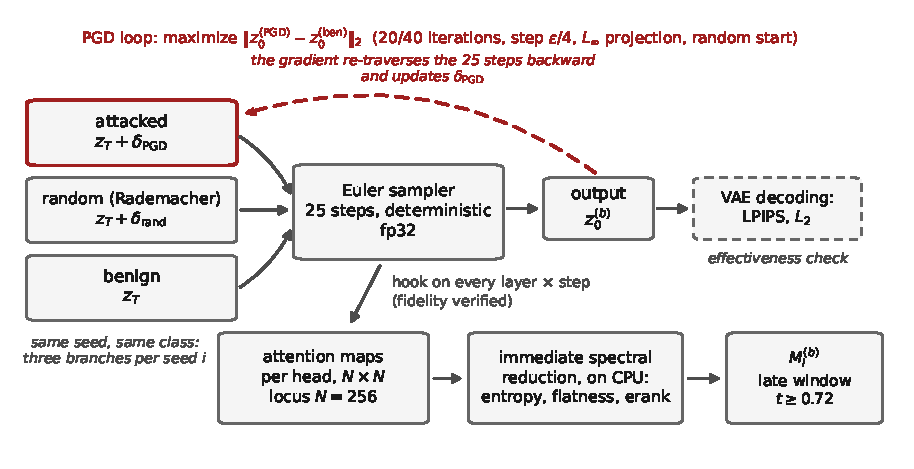
\includegraphics[width=0.7\textwidth]{fig_pipeline.pdf}
  \caption{Attack and measurement pipeline, identical for the two models. Three branches per seed share the initial noise and the class; PGD maximizes the output displacement through the 25 Euler steps and never reads the attention; hooks reduce every map, per head, to spectral scalars on the CPU; the registered statistics live on the late window $t \ge 0.72$ of the $N{=}256$ locus.}
  \label{fig:pipeline}
\end{figure*}

\subsection{Pilot Study}

The pilot is exploratory and reported for what it decided; its aggregates are full-trajectory means over the 25 steps, about half of the late-window values on which the confirmatory study is defined. It was pre-registered before its data were generated: $n{=}100$ paired seeds, $\varepsilon{=}0.05$, 20 iterations, $K{=}3$ Rademacher draws per seed, and a two-part pass rule per metric (mean contrast at least two standard errors in the pre-fixed direction and a one-sided Wilcoxon signed-rank test at $p<0.05$).

\begin{table}[t]
  \caption{Pilot outcomes on the $N{=}256$ locus (full trajectory, $n{=}100$, $\varepsilon{=}0.05$, 20 iterations). Mean contrast, standard error and Cohen's $d$; the entropy is an absolute shift, the two spectral metrics a drop. All six pass with Wilcoxon $p<10^{-9}$.}
  \label{tab:pilot}
  \centering
  \begin{small}
    \setlength{\tabcolsep}{3pt}
    \begin{tabular}{lcccccc}
      \toprule
       & \multicolumn{3}{c}{DiT} & \multicolumn{3}{c}{UNet} \\
      \cmidrule(lr){2-4} \cmidrule(lr){5-7}
      metric & mean & SE & $d$ & mean & SE & $d$ \\
      \midrule
      row entropy       & 0.010 & 0.001 & 1.24 & 0.011 & 0.001 & 1.37 \\
      spectral flatness & 0.006 & 0.001 & 0.93 & 0.004 & 0.001 & 0.77 \\
      effective rank    & 0.018 & 0.002 & 1.09 & 0.023 & 0.002 & 1.09 \\
      \bottomrule
    \end{tabular}
  \end{small}
  \vspace{-0.3cm}
\end{table}

All three metrics pass on both models (Table~\ref{tab:pilot}), with Cohen's $d$ between 0.77 and 1.37. The random branch leaves the metrics where they are: it changes the effective rank by less than 0.001, against drops from benign of 0.018 and 0.022 under attack, from benign levels of 0.41 (DiT) and 0.20 (UNet). The attack is perceptually effective: the LPIPS~\cite{zhang2018unreasonable} distance between decoded benign and perturbed outputs is 0.55 (DiT) and 0.54 (UNet), 15 to 20 times the random branch against a pre-fixed threshold ratio of 1.5, with output $L_2$ displacements of 45.2 and 44.7. Without this check a null attention result would be ambiguous between an unresponsive attention and an invisible attack.

\textbf{Differential FID.} We had registered a differential FID, $\mathrm{ddFID} = \mathrm{dFID}_{\mathrm{PGD}} - \mathrm{dFID}_{\mathrm{rand}}$ against the real reference, as a candidate attack indicator with a positive-direction pass rule. The outcome was the opposite: PGD \textit{lowers} the FID, with ddFID $-15.9$ [$-19.4$, $-11.0$] for the DiT and $-17.7$ [$-20.7$, $-12.3$] for the UNet (bootstrap 95\% intervals; absolute FID at $n{=}1000$ from 107.8 to 91.7 and from 136.1 to 119.0, upward-biased by the small $n$). Decomposing the FID into its mean and covariance terms attributes 64\% (DiT) and 73\% (UNet) of the drop to the mean term, while the batch diversity, the trace of the feature covariance, changes by $-1.2\%$ and $+2.5\%$: the attack moves individual samples by a large amount while pulling the batch mean toward the real reference, without mode collapse. A set-level distance is therefore not an adequate indicator of a per-sample displacement attack, and the metric was dropped.

\textbf{Metric election.} The registered rule elected the metric with the largest standardized effect, with a tie-break within 15\% in favor of the spectral measure. The two models disagreed: on the DiT the entropy ($d{=}1.24$) and the effective rank ($d{=}1.09$) were within 15\%, so the tie-break elected the effective rank; on the UNet the entropy ($d{=}1.37$) exceeded the effective rank ($d{=}1.09$) by more. We resolved the disagreement by a design decision, fixed in the confirmatory pre-registration before its data existed: the effective rank is primary, because its direction of effect is univocal (the entropy shifts in both directions, with signed means below 0.002 in modulus against absolute shifts near 0.011), its $d$ is identical on the two models, and it is the quantity an attack aimed at the rank would target (ours is not). The pilot also showed the contrast concentrating in the final steps (full-trajectory 0.018 and 0.023 against late-window 0.033 and 0.046) and a different depth location, the UNet contrast almost entirely in the decoder and the DiT contrast spread over block 0 and the deep blocks; with $n{=}100$ the standard error of $d$ is about 0.13, too large to compare the models.

\subsection{Confirmatory Design}\label{sec:design}

The design was frozen in a pre-registration document, versioned in the public repository before any confirmatory data existed, with two pre-launch implementation amendments registered the same way (Appendix~\ref{app:controls}); seeds are disjoint from the pilot by construction. Two co-primary hypotheses are tested two-sided, with no a-priori sign for a cross-model difference.

\textbf{Co-primary A, magnitude.} The paired cross-model difference of the mean late-window contrast on the shared locus,
\begin{equation}\label{eq:delta-a}
  \Delta_A = \frac{1}{n} \sum_{i=1}^{n} \bigl( c_i^{(\mathrm{DiT})} - c_i^{(\mathrm{UNet})} \bigr),
\end{equation}
in effective-rank units. The scale is absolute by design: dividing by each model's benign level would re-encode the twofold benign gap, and the pilot already showed that the sign of the difference depends on the locus (on all layers the DiT contrast, 0.018, exceeds the UNet's, 0.010). Both framings are reported descriptively next to $\Delta_A$, as the pre-registration requires.

\textbf{Co-primary B, structure.} For each seed, the share of the clamped per-layer contrast that falls on the input side of the network, in excess of the share expected under a uniform spread,
\begin{equation}\label{eq:share}
  S_i = \frac{\sum_{l \in \mathrm{in}} \max(c_{l,i}, 0)}{\sum_{l} \max(c_{l,i}, 0)} - \frac{L_{\mathrm{in}}}{L},
\end{equation}
with the input side the two encoder blocks of the UNet ($L_{\mathrm{in}}/L = 2/5$) and the first half of the DiT (blocks 0 to 5, $6/12$). Under a within-seed permutation of the layers $\mathbb{E}[S_i] = 0$ exactly. The co-primary is the paired excess
\begin{equation}\label{eq:delta-b}
  \Delta_B = \frac{1}{n} \sum_{i=1}^{n} \bigl( S_i^{(\mathrm{DiT})} - S_i^{(\mathrm{UNet})} \bigr),
\end{equation}
over the seed pairs whose clamped mass is positive for both models; the analysis is repeated with higher exclusion floors, with the DiT boundary moved by one block, and in a second version where the layer contrasts are averaged over seeds before the clamp. An independent review of the design before the freeze replaced the original version of B, an entropy of the layer profile compared with a within-seed shuffle, which is permutation-invariant and hence degenerate, with the positional share above.

\textbf{Margins.} The study is over-powered ($|\Delta|/\mathrm{SE} \approx 9$ forecast from the pilot), so the verdict rests on a smallest effect size of interest~\cite{lakens2017equivalence}. SESOI-A $= 0.010$ is a quarter of the pooled late-window fingerprint of the two models in the pilot, 0.039: above it, a difference would justify architecture-specific attacks. SESOI-B $= 0.10$ sits just above the largest effect attributable to the one arbitrary choice in $S_i$, the half-depth cut of the DiT, whose displacement by one block shifts the neutral fraction by $1/12 \approx 0.083$; the UNet boundary is architectural and not movable, so the alternative margin of 0.20 (its one-block step, $1/5$) was considered and rejected. The pilot's late-window values of $\Delta_B$, 0.16 per seed and 0.12 on the seed-mean profile, cleared 0.10 and not 0.20; we return to this contingency in the limitations.

\textbf{Family and verdict rule.} The procedure of \citet{holm1979simple} at $\alpha = 0.05$ over five members: co-primary A, co-primary B, a dose-response member (the paired difference of per-seed slopes of the contrast on $\log \varepsilon$), and the entropy and flatness echoes of A. Each member contributes one p-value, the larger of a paired t-test and a Wilcoxon signed-rank test. Per co-primary the outcome is one of three: (1) rejection after Holm, $|\mathrm{estimate}| \ge$ SESOI and the matched-quality control passed, hence distinguishable on that axis; (2) rejection with $|\mathrm{estimate}| <$ SESOI, hence statistically detectable but below the threshold of interest; (3) no rejection, decided by two one-sided tests~\cite{schuirmann1987comparison}, equivalent within the margin if the 90\% confidence interval lies inside $\pm$SESOI and inconclusive otherwise. The architectures are distinguishable if and only if at least one co-primary reaches outcome (1); the other three members corroborate and cannot decide.

\textbf{Grid, sampling and controls.} Budgets $\varepsilon \in \{0.01, 0.02, 0.05, 0.1\}$ with 0.05 primary; $n{=}500$ seeds per configuration with distinct class labels 0 to 499, shared across models and budgets, with shared noise and shared attack initialization; 40 iterations; one Rademacher draw per seed, since in the pilot the variation across draws was about 5\% of the variation across seeds. Sharing seeds is efficient: the pilot cross-model correlation of contrasts was $+0.56$, which lowers the standard error of the paired difference by about 32\%. Five controls were registered with pass criteria. The \textit{matched-quality} control compares DiT@FID95 with the final DiT and with the UNet at the primary budget: an effect is attributable to the architecture only if DiT@FID95 is equivalent to the final DiT within the relevant SESOI and keeps the sign of the DiT--UNet difference, the outcome being declared ambiguous otherwise. The others are \textit{transfer} to 50 and 100 sampler steps (same sign, Holm-significant, magnitude within a factor two of the primary); \textit{attack comparability} (per-budget ratio of output $L_2$ displacements between models within $[0.8, 1.25]$); \textit{saturation} (contrast at $\varepsilon{=}0.1$ at least twice that at 0.05); and an \textit{iteration plateau} over 20, 40 and 80 iterations (gap between 80 and 40 within 10\%). The analysis code was finalized before any cross-model statistic was computed, validated on the pilot's disjoint seeds, and embeds its own version identifier in the output.

% ------------------------------------------------------------------------------
% RESULTS
% ------------------------------------------------------------------------------
\section{Results}\label{sec:results}

Unless stated otherwise, every number below is at $\varepsilon{=}0.05$, on the late window, on the shared $N{=}256$ locus, over 500 seeds.

\subsection{Confirmatory Results}\label{sec:confirmatory}

\paragraph{The fingerprint at confirmatory scale.} The collapse contrast of Eq.~\eqref{eq:contrast} is $+0.035$ for the DiT and $+0.041$ for the UNet: under attack the effective rank of the attention maps drops more than under the Rademacher control of equal budget. The effect is large and stable across seeds, with Cohen's $d$ of 1.25 and 1.32. The two models collapse from different benign levels, 0.47 and 0.26. Figure~\ref{fig:dose-temporal} shows that the contrast grows with the budget (DiT 0.005, 0.011, 0.035 and 0.096 at the four budgets; UNet 0.004, 0.011, 0.041 and 0.114) and that it accumulates in the final steps: at the first step the cross-model difference has the opposite sign ($+0.005$, with disjoint confidence intervals), and the whole gap sits inside the late window.

\begin{figure*}[t]
  \centering
  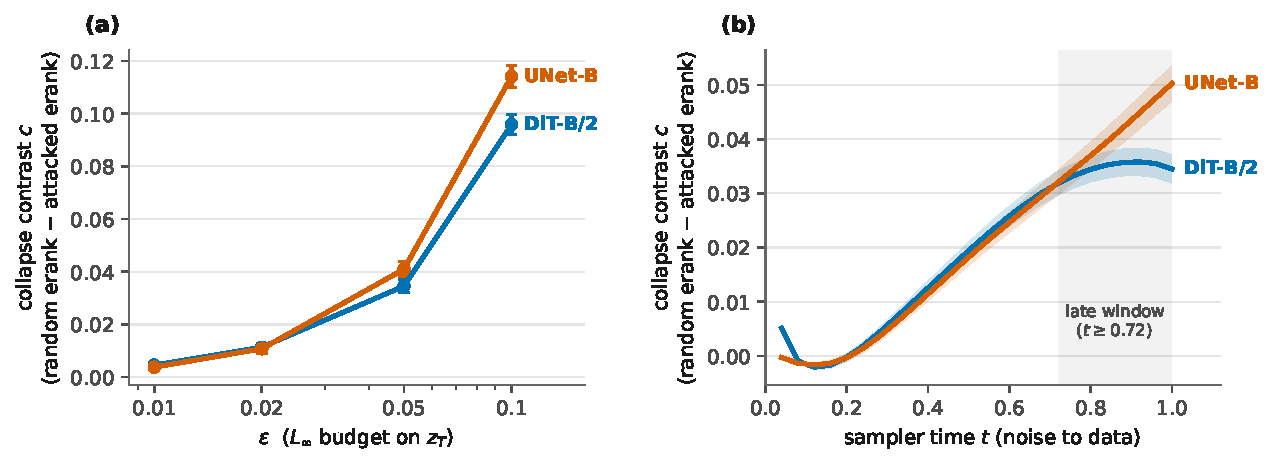
\includegraphics[width=0.8\textwidth]{fig_dose_temporal.pdf}
  \caption{(a) Dose response of the late-window collapse contrast against the budget $\varepsilon$ (500 seeds, bars are 95\% confidence intervals). (b) Temporal profile of the contrast along sampler time at $\varepsilon{=}0.05$, averaged over the locus and the seeds, with 95\% bands; the shaded zone is the late window $t \ge 0.72$ on which the confirmatory measures are defined.}
  \label{fig:dose-temporal}
\end{figure*}

\paragraph{Co-primary A: magnitude.} $\Delta_A = -0.006$ with standard error 0.001 (Table~\ref{tab:family}): the UNet's rank reduction is larger. The null hypothesis is rejected after Holm ($p = 1.77{\times}10^{-6}$), and the two one-sided tests pass, since the 90\% confidence interval $[-0.009, -0.004]$ lies inside $\pm 0.010$. This is the second of the three registered outcomes: the difference is statistically detectable but below the smallest effect size of interest. On a quantity bounded in $[0, 1]$ this is a difference at the third decimal, about a sixth of the fingerprint itself and below a margin set at a quarter of it; with 500 paired seeds the test resolves differences this small, which is why the verdict rests on the margin rather than on the p-value. Three framings, all descriptive, qualify the statement and must be read with it. In proportion to its own benign level the UNet is about twice as susceptible, 0.15 vs 0.07. On the locus extended to all layers the DiT keeps 0.035 (its locus already covers all 12 blocks) while the UNet falls to 0.020, because the rank barely moves in its 64- and 16-token blocks, and the difference becomes $+0.015$ with the sign flipped. On the full trajectory the difference shrinks to $-0.001$ ($p = 0.064$), and at the two smaller budgets it is $+0.001$ ($p = 0.15$ and $p = 0.70$), where the attack-comparability criterion is also out of band. The below-margin conclusion holds on the pre-registered absolute scale and locus, not on every framing.

\begin{table*}[t]
  \caption{The Holm family ($\alpha{=}0.05$): estimate, bootstrap 95\% interval, Holm-adjusted p-value and margin. $\Delta_A$ and $\Delta_B$ are DiT minus UNet. B also passes in its second version, on the seed-mean profile ($+0.13$).}
  \label{tab:family}
  \centering
  \begin{small}
    \begin{tabular}{lccc}
      \toprule
      member & estimate [95\% CI] & $p_{\mathrm{Holm}}$ & margin \\
      \midrule
      A, magnitude  & $-0.006$ [$-0.009$, $-0.004$] & $1.77{\times}10^{-6}$ & inside $\pm 0.010$ \\
      B, structure  & $+0.18$ [0.16, 0.20] & $1.92{\times}10^{-59}$ & beyond 0.10 \\
      dose response & $-0.008$ [$-0.010$, $-0.007$] & $2.51{\times}10^{-25}$ & -- \\
      entropy echo  & $+0.003$ [0.001, 0.004] & $5.24{\times}10^{-4}$ & -- \\
      flatness echo & $+0.004$ [0.003, 0.005] & $1.20{\times}10^{-12}$ & -- \\
      \bottomrule
    \end{tabular}
  \end{small}
  \vspace{-0.3cm}
\end{table*}

\paragraph{Co-primary B: structure.} $\Delta_B = +0.18$ over 478 seed pairs: the DiT places about 18 percentage points more of its contrast toward the input side than the UNet, relative to a uniform spread. Twenty-two pairs are excluded because the clamped mass is zero on at least one side (5 DiT seeds, 19 UNet seeds, two in common). The second version, with layer contrasts averaged before the clamp, gives $+0.13$; both exceed SESOI-B $= 0.10$. The within-model corroborations agree: the UNet decoder exceeds its encoder by 0.06 of mean per-layer contrast, and the DiT's block 0 carries a per-seed excess share of 0.10. The estimate stays at 0.18 for every exclusion floor from 0 to 0.033, and moving the DiT boundary by one block gives 0.24 (blocks 0 to 4 as input side) or 0.21 (blocks 0 to 6). With the rejected alternative margin of 0.20 neither version would pass (0.18 and 0.13).

\paragraph{The matched-quality control.} On magnitude the control passes: DiT@FID95 differs from the final DiT by $-0.002$, equivalent within $\pm 0.010$, and keeps the sign against the UNet. On structure it does not: DiT@FID95 differs from the final DiT by $-0.12$, with a 90\% interval $[-0.140, -0.103]$ entirely outside $\pm 0.10$ (483 pairs). Two checkpoints of the same architecture differ in localization comparably to the two architectures, which is the case the pre-registration declared ambiguous: the registered reading is that the localization tracks training convergence. Figure~\ref{fig:localization} shows where. In DiT@FID95 the input-side peak is at block 3 (0.047) and block 0 is nearly silent (0.001); in the final DiT the input-side peak is at block 0 (0.047), where an attention sink sits. On the late window the benign rows of the final DiT's block 0 have normalized entropy 0.91 with effective rank 0.10, the signature of rows that are not uniform yet share the same few anchor tokens, whereas in DiT@FID95 the same rows are still uniform (entropy 1.00, effective rank 0.01). The sink is absent in DiT@FID95 and present in the final DiT, and this observation is what the convergence reading rests on.

\begin{figure*}[t]
  \centering
  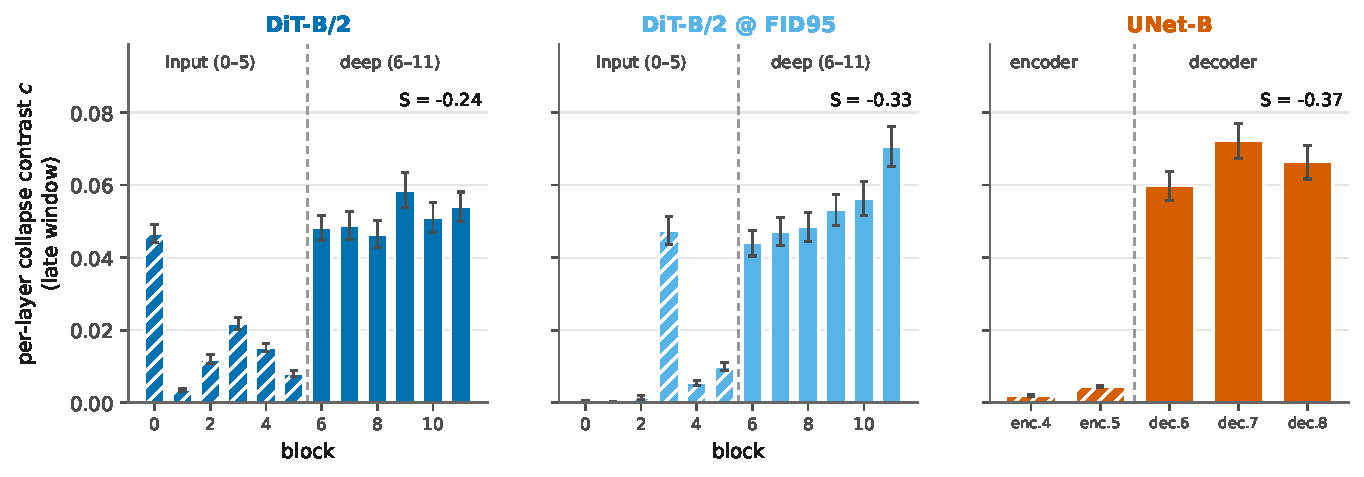
\includegraphics[width=0.92\textwidth]{fig_localization.pdf}
  \caption{Per-layer collapse-contrast profiles at $\varepsilon{=}0.05$ on the late window (bars: 95\% confidence intervals; hatching: input side). $S$ is the input-side share in excess of the neutral fraction, computed on the mean profiles: it is negative for all three checkpoints ($-0.24$, $-0.33$, $-0.37$), since the fingerprint leans toward the deep layers everywhere, and its difference between models is the second version of co-primary B. The intermediate DiT checkpoint (center) has not yet developed the block-0 peak of the final DiT (left).}
  \label{fig:localization}
\end{figure*}

\begin{table*}[t]
  \caption{Registered controls at $\varepsilon{=}0.05$ (budget-specific where indicated). The attack-comparability ratio is the DiT/UNet ratio of output $L_2$ displacements.}
  \label{tab:controls}
  \centering
  \begin{small}
    \begin{tabular}{llc}
      \toprule
      control & value & outcome \\
      \midrule
      comparability, $\varepsilon{=}0.01/0.02/0.05/0.1$ & 1.26 / 1.13 / 1.01 / 0.99 & out of band at 0.01 \\
      transfer, 50 steps: $\Delta_A$, $\Delta_B$ & $-0.011$ (1.72$\times$), $+0.18$ & passed \\
      transfer, 100 steps: $\Delta_A$, $\Delta_B$ & $-0.013$ (2.06$\times$), $+0.17$ & A beyond 2$\times$ \\
      saturation, $c(0.1)/c(0.05)$ & 2.78$\times$ both models & not saturated \\
      iteration plateau, 80 vs 40 & 2.2\% (DiT), 0.6\% (UNet) & passed \\
      matched quality, A & $-0.002$, inside $\pm 0.010$ & passed \\
      matched quality, B & $-0.12$, outside $\pm 0.10$ & not passed \\
      \bottomrule
    \end{tabular}
  \end{small}
  \vspace{-0.3cm}
\end{table*}

\paragraph{The other members and the controls.} The dose-response member is $-0.008$ and Holm-significant: the UNet contrast grows faster with the budget. By the registered rule it corroborates and cannot decide. The entropy and flatness echoes, $+0.003$ and $+0.004$, are both significant, but their signs do not read the same way: the flatness echo uses the same contrast as A and says the DiT is more affected, the opposite of the effective rank, while the entropy echo is defined on absolute shifts and carries no sign comparison; the secondary metrics do not single out one more susceptible model. Table~\ref{tab:controls} collects the controls. The attack is comparably successful on the two models at the three larger budgets (ratios 1.13, 1.01, 0.99) and slightly more successful on the DiT at $\varepsilon{=}0.01$ (1.26, just outside the band). Under transfer to 50 and 100 steps both co-primaries keep their sign and significance; $\Delta_A$ grows to $-0.011$ and $-0.013$, and at 100 steps it exceeds the factor-two band in the stronger direction, while $\Delta_B$ stays at $+0.18$ and $+0.17$. The contrast at $\varepsilon{=}0.1$ is 2.78 times that at 0.05 on both models, so the primary budget is not saturated. Doubling the iterations from 40 to 80 moves the contrast by 2.2\% (DiT) and 0.6\% (UNet). The per-seed contrasts of the two models correlate at 0.52, against the 0.56 anticipated from the pilot, confirming the precision gain of the paired design. Figure~\ref{fig:qualitative} shows one paired seed.

\begin{figure}[t]
  \centering
  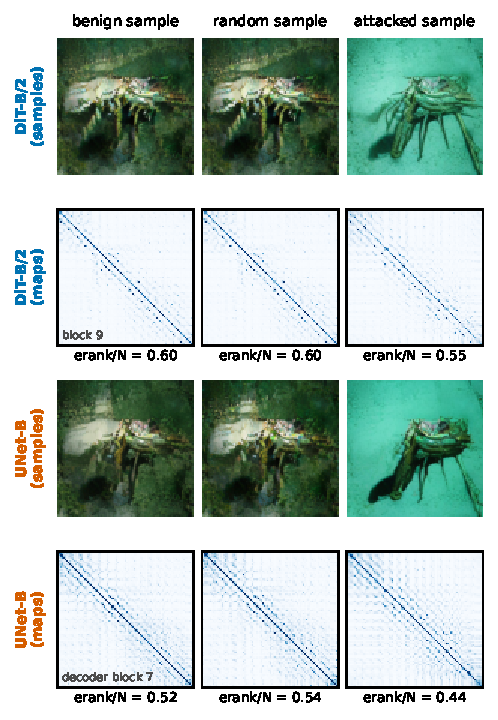
\includegraphics[width=0.9\columnwidth]{fig_qualitative.pdf}
  \caption{One paired seed (seed 123, chosen by a frozen median-rank rule) at $\varepsilon{=}0.05$: decoded samples and head-averaged attention maps at the last sampler step, on each model's maximum-contrast layer (block 9 of the DiT, decoder block 7 of the UNet). Under each map, the normalized effective rank: 0.60, 0.60 and 0.55 for the DiT, 0.52, 0.54 and 0.44 for the UNet on the benign, random and attacked branches. The attacked samples remain plausible images of the same class.}
  \label{fig:qualitative}
\end{figure}

\paragraph{Verdict.} Under the pre-registered decision rule the two architectures are not distinguishable. The magnitude difference is statistically detectable ($\Delta_A = -0.006$, Holm-adjusted $p = 1.77{\times}10^{-6}$) but lies below the smallest effect size of interest on the absolute effective-rank scale the analysis was registered on (SESOI-A $= 0.010$); relative to each model's benign level the UNet responds about twice as strongly (0.15 vs 0.07) and on the locus extended to all layers the sign flips ($+0.015$), both descriptively. The structural difference is wide ($\Delta_B = +0.18$ against SESOI-B $= 0.10$) but cannot be attributed to the architecture: the same DiT at a less converged checkpoint (DiT@FID95) differs from the final DiT by $-0.12$, beyond the margin. The registered reading of this case, declared ambiguous in the pre-registration, is that the localization tracks training convergence. This is one of the two outcomes the design was built to interpret, not a missed result.

\subsection{Exploratory Analyses}\label{sec:exploratory}

The analyses in this section are post hoc, outside the pre-registered family, without multiplicity correction, and descriptive.

\begin{figure*}[!t]
  \centering
  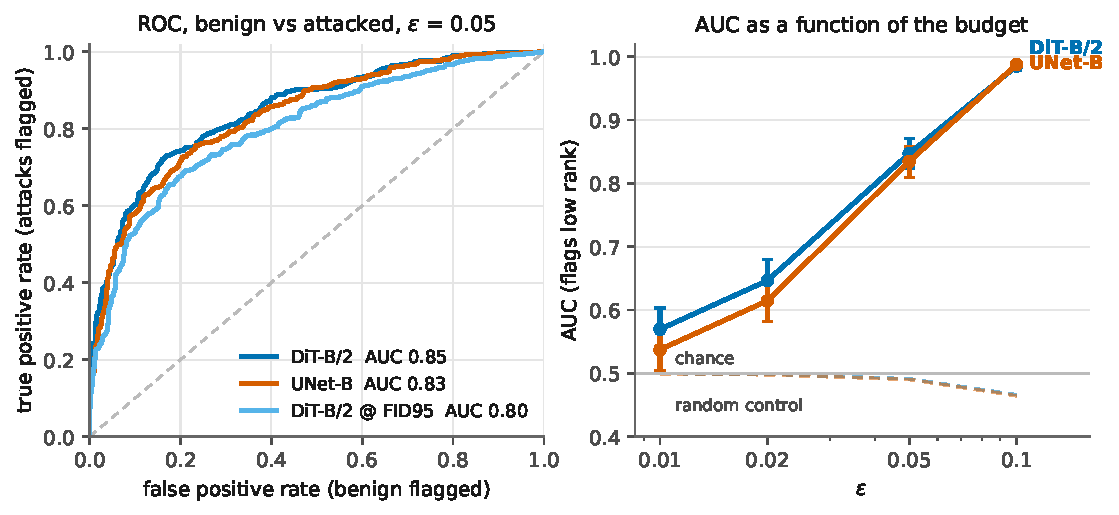
\includegraphics[width=0.74\textwidth]{fig_detector.pdf}
  \caption{The late effective rank as a detector (exploratory). Left: ROC curves at $\varepsilon{=}0.05$ for the DiT, the UNet and DiT@FID95. Right: AUC against the budget with bootstrap 95\% intervals; dashed, the random control, at chance.}
  \label{fig:detector}
\end{figure*}

\begin{figure*}[!t]
  \centering
  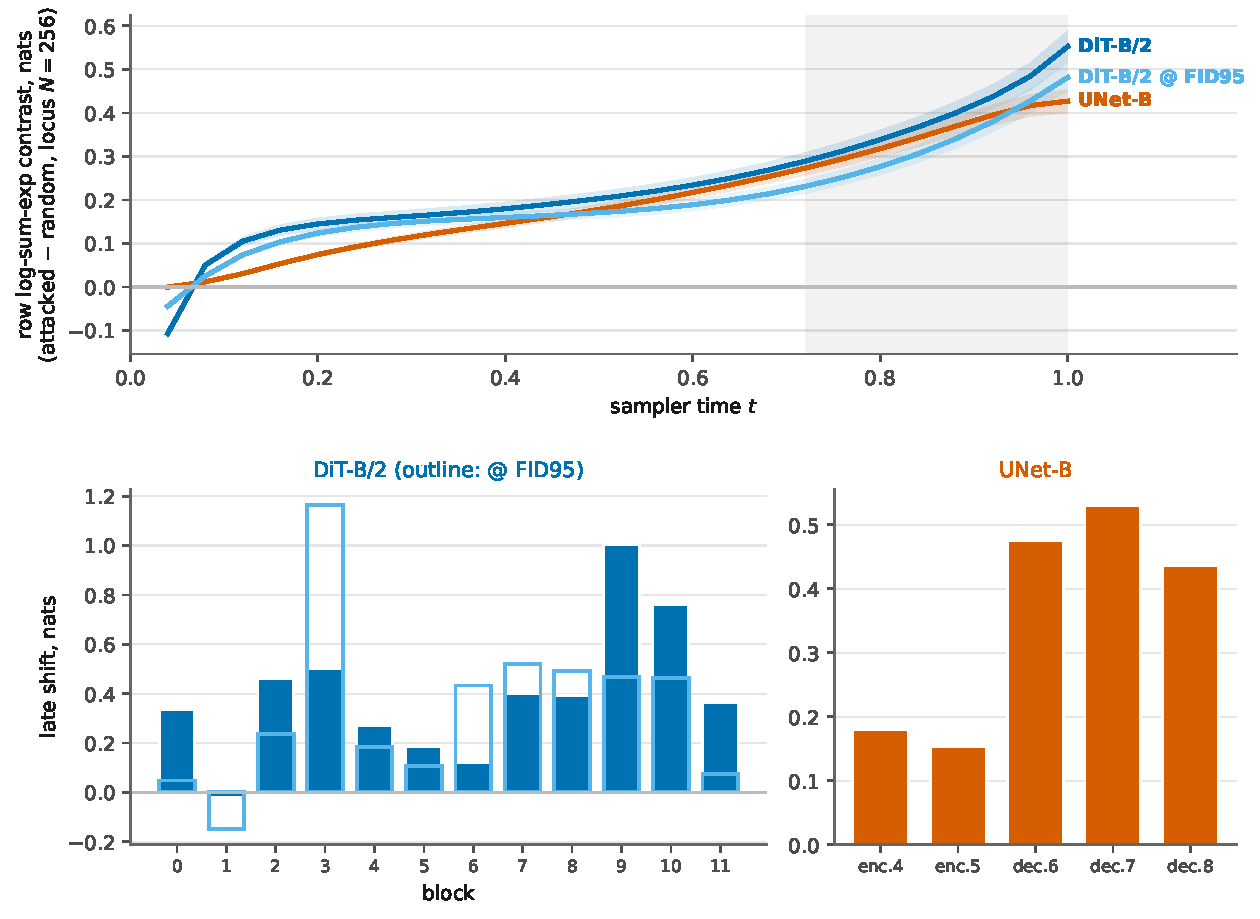
\includegraphics[width=0.62\textwidth]{fig_energy.pdf}
  \caption{Softmax energy (exploratory). Top: row log-sum-exp contrast between the attacked and the random branch along sampler time for the three checkpoints (bands: 95\% intervals; shaded: late window). Bottom: late per-layer shift, DiT with DiT@FID95 as outline (left) and UNet (right).}
  \label{fig:energy}
\end{figure*}

\paragraph{The fingerprint as a detector.} We score each sample by its late-window effective rank on the locus and flag it when the score is low. The AUC against the benign branch grows with the budget: 0.85 (DiT) and 0.83 (UNet) at $\varepsilon{=}0.05$, 0.57 and 0.54 at 0.01, 0.99 for both at 0.1, with 0.80 for DiT@FID95 at 0.05 (Figure~\ref{fig:detector}). The random branch stays at chance, with AUC between 0.46 and 0.50 at every budget: the detector responds to the attack, not to the size of the perturbation. Operating points set at the fifth percentile of the same benign set are in-sample and optimistic by construction. The only out-of-sample evidence is the transfer of the threshold expressed in benign z-units: calibrated on one model and applied to the other without refitting, it keeps a false-positive rate of 4\% (DiT to UNet), 6\% (UNet to DiT) and 4.8\% (DiT to DiT@FID95), and at $\varepsilon{=}0.1$ it detects 92.4\% and 93.6\% of the attacked samples. What transfers is the position relative to the benign distribution rather than the raw threshold.

\paragraph{Softmax energy.} Following the energy-based reading of logits~\cite{grathwohl2020your}, we take the row log-sum-exp of the attention logits, averaged over rows, heads, locus layers and late steps, with energy $E = -\mathrm{LSE}$. Under attack the LSE rises on all three checkpoints: the contrast with the random branch is $+0.40$ nats for the DiT (benign level 10.51), $+0.35$ for the UNet (6.94) and $+0.34$ for DiT@FID95 (10.38), with Cohen's $d$ of 1.36, 1.48 and 1.37, the same order as the rank contrast; the random branch moves by less than 0.01 nats. The energy therefore falls, the direction known for untargeted attacks on classifiers~\cite{mirza2024shedding}. The raw levels are not comparable across backbones; the within-model shifts are. About two thirds of the shift comes from the row's peak logit (69\%, 66\% and 70\%), the rest from the log tail mass. The per-layer profile echoes the rank localization: the UNet shift concentrates in the decoder, the DiT shift peaks at block 9 (1.00 nats) as the rank contrast does, and DiT@FID95 peaks at block 3 (1.16) with block 0 at 0.05. The shift follows the dose on the DiT, with $d$ of 0.35, 0.61, 1.36 and 2.19 at the four budgets and an energy-only AUC of 0.96 at the largest, while the random control stays at chance. Energy and rank move together seed by seed: the Pearson correlation between the energy shift and the rank contrast is 0.59 (DiT), 0.68 (UNet) and 0.53 (DiT@FID95). As a detector at $\varepsilon{=}0.05$ the energy alone reaches AUC 0.79, 0.88 and 0.83, and the sum of the two benign-normalized z-scores 0.86, 0.89 and 0.86, against 0.85, 0.83 and 0.80 for the rank alone. Figure~\ref{fig:energy} shows the time course and the layer profiles.

\paragraph{Additional checks run after the thesis.} Two checks, run after the thesis was defended and not pre-registered, address two objections. First, the FID decrease could be an artifact of the Inception feature space and its alignment with ImageNet. On the 500 confirmatory seeds we recomputed the three-branch FID in Inception, CLIP and DINOv2 feature spaces: the attacked branch lowers the FID in all three, by 7.9\%, 7.1\% and 4.6\% for the DiT and 7.9\%, 5.4\% and 4.9\% for the UNet, with the mean term carrying at least 66\% of the drop everywhere and the random branch unmoved. Second, the attack could be a better ODE solver in disguise, moving the sample toward the accurate solution of the flow. On 200 confirmatory seeds we compared the attack displacement with the correction that Heun's method at 25 steps or Euler at 100 steps applies to the 25-step Euler output. The cosine between the attack direction and the 100-step correction is 0.05 (DiT) and 0.08 (UNet), against 0.99 between the two solvers, and the attack displacement is about eight times larger than the correction. In no seed does the attack bring the output closer to the 100-step solution, and on the late window the accurate solver \textit{raises} the effective rank by about a tenth of the drop observed under attack. On the pilot batch the two solvers recover between a third and a half of the attack's FID decrease (0.33 and 0.38 of the drop for Euler at 100 steps, 0.35 and 0.45 for Heun), with the same mean-dominated signature, so the direction toward higher-density regions is partly shared with an accurate solver while the attention fingerprint is specific to the attack.

% ------------------------------------------------------------------------------
% DISCUSSION
% ------------------------------------------------------------------------------
\section{Discussion and Conclusions}\label{sec:discussion}

\textbf{A directional, late fingerprint.} The attack leaves a fingerprint that is specific to its direction, since the random perturbation of equal budget leaves the metrics untouched, and late, since it accumulates in the last sampler steps; over the full trajectory the cross-model difference loses significance ($p = 0.064$). The fingerprint does not separate the two models under the pre-registered rule: the magnitude difference is detectable but below the registered margin on the absolute scale ($-0.006$ against 0.010, with the UNet about twice as susceptible relative to its benign level and the sign reversed on the all-layer locus), and this is one of the two outcomes the design was built to interpret. Our account of the non-separation is that what we measure stays confined to the attention of each architecture, which in the DiT is the only spatial-mixing mechanism and in the UNet coexists with convolutions; the two systems also start from different benign geometries (0.47 against 0.26), and the comparison against the margin is conducted in raw effective-rank units on the shared locus, while the relative scale tells a different story (Section~\ref{sec:confirmatory}).

\textbf{Against the pixel-space intuition.} The hypothesis that motivated this measurement was that adversarial noise is high-rank and off-manifold: a dense pattern of $\pm\varepsilon$ signs is, as a matrix, generically full rank, and the idea that adversarial examples occupy low-probability regions goes back to \citet{szegedy2013intriguing}. Our measurement through the sampler reports the opposite: under attack the effective rank of attention goes down and the maps end up more concentrated. The response is emergent, since the attack does nothing but displace the output and never reads the maps. We have not studied how PGD acts in pixel space in general; we compared a hypothesis with an observation in a different and controlled setting, where the perturbation acts on the initial noise and traverses a differentiable sampler in latent space.

\textbf{Localization tracks convergence.} At equal architecture, the structural difference between two checkpoints stopped at different times is comparable in modulus to the difference between the architectures ($-0.12$ against $+0.18$), and the attention sink at block 0 that anchors the final DiT's input-side peak is absent in DiT@FID95. The data exclude attributing the localization to the architecture; the reading we propose is that the depth at which the fingerprint concentrates is a property of training maturity. This suggests a methodological check for work that interprets depth localizations as architectural properties: compare the same network at different checkpoints before attributing a localization to the design.

\textbf{Energy and FID toward high-density regions.} Two independent measures agree on a direction. The FID of attacked samples falls relative to the random control because the mean of their features moves toward the real reference while the covariance does not collapse, and the attention energy falls while the rows concentrate; the two co-vary seed by seed. We interpret this agreement as a push toward regions the model treats as more probable, the inference-time counterpart of what \citet{briglia2025adversarial} observe under adversarial training, where trajectories cluster onto modes without mode collapse; here the weights do not change. The solver check sharpens this interpretation: an accurate solver shares part of the FID direction but produces the opposite rank response, so the attention fingerprint belongs to the attack rather than to the integration error of the sampler. For the same reason a set-level distance is a poor detector of a displacement attack, while a local spectral statistic in standardized units transfers across the three checkpoints with 4\% to 6\% false positives. The fingerprint is likely a property of the attack observed through each model's attention, which would explain why it transfers across the three checkpoints without separating the architectures under the pre-registered rule.

\textbf{Limitations.} (i) The flip augmentation is applied in latent space, where the VAE does not commute with reflection: the two routes to the flipped image agree at 19.2~dB against 24.8 for reconstruction; the defect is symmetric between the models and no retraining was done. (ii) The convergence reading rests on a single control checkpoint, on the DiT side only, trained in a different regime (batch 64 against 16, stopped at 150\,000 steps); whether a UNet at intermediate maturity behaves the same way is unknown. (iii) At 100 sampler steps co-primary A leaves the factor-two band in the stronger direction ($-0.013$ against $-0.006$): the formal criterion fails while the effect strengthens, so the magnitude is not stable in sampler length. (iv) The dose response does not saturate within the grid (2.78$\times$ at double budget), so where the phenomenon flattens is unknown. (v) At $\varepsilon{=}0.01$ the displacement ratio is 1.26, outside the registered band, and comparisons at that budget are weaker. (vi) The FID protocol is internal to this work: the absolute values are not comparable externally and FID is a convergence indicator only. (vii) The below-threshold conclusion holds in the registered units and on the registered locus; relative to benign the UNet's susceptibility is about double (0.15 vs 0.07) and on all layers the difference changes sign ($+0.015$). (viii) The structural outcome depends on the margin: with the rejected alternative of 0.20, co-primary B would pass in neither version (0.18 and 0.13). (ix) The training path is asymmetric (bf16, cloud GPU, cosine schedule, clipping and weight decay for the UNet); these differences do not touch the attack or the measurement, which share precision, hardware and seeds. (x) The shared locus matches token count, not depth: five UNet blocks against twelve DiT blocks at different positions. (xi) A wide quality gap remains between the final models (68.67 against 99.14); the matched-quality control exists for this reason. (xii) Per-seed means rest on 1152 cells for the DiT and 160 for the UNet, with twelve against four heads, without correction. (xiii) The confirmatory random branch uses one Rademacher draw per seed. (xiv) The detector's detection rates are in-sample; the z-unit transfer is its only out-of-sample check. (xv) The study covers one pair of models at size B, self-attention only and class conditioning only; nothing here licenses generalization to other backbones, other scales or cross-attention.

\textbf{Future work.} The effective rank was elected in part because it is differentiable and moves in a constant direction, which makes it attackable: an objective that touches the attention would test whether the fingerprint can be driven or hidden. Same-regime convergence controls, on both the DiT and the UNet side, would resolve limitation (ii). The measurement chain assumes nothing about the architecture beyond readable attention layers and could be applied unchanged to other open-weight models; text-image cross-attention is the natural extension.

\bibliography{references}
\bibliographystyle{dlaiml2025}

% ------------------------------------------------------------------------------
% APPENDICES
% ------------------------------------------------------------------------------
\clearpage
\appendix

\section{UNet Training History and Asymmetries}\label{app:training}

Table~\ref{tab:runs} lists the training runs behind the two final checkpoints and the control checkpoint. The DiT trained in fp16 on the local GPU without weight decay, clipping or intervention. The UNet in fp16 did not: the loss became non-finite at about 94\,000 steps, and a second attempt with gradient clipping failed earlier, at about 79\,000, because the overflow is in the forward pass, where clipping has no effect. The overflow is in the $QK^\top$ attention logits: the scale $1/\sqrt{d}$ was applied after the product, and the unscaled product exceeded the fp16 range. A first fix (scale $q$ and $k$ by $d^{-1/4}$ before the product, softmax in fp32, plus the abort guard) delayed the overflow to about 192\,000 steps and, with weight decay, to about 234\,000; the definitive fix computes the scores and the softmax in fp32 with autocast disabled. Since the local GPU has no native bf16 (an RDNA 2 part, on which bf16 autocast runs about five times slower than fp32), the UNet was restarted from scratch in bf16 on a cloud RTX 3090.

\begin{table}[H]
  \caption{Training runs. All at batch 16, learning rate $10^{-4}$, EMA 0.9999, except the first (batch 64), whose 150\,000-step checkpoint is DiT@FID95. wd: weight decay 0.01; clip: gradient clipping at norm 1.0; guard: automatic abort after 500 consecutive non-finite losses; cos.: cosine schedule; *: attention with split scaling before the product and fp32 softmax.}
  \label{tab:runs}
  \centering
  \begin{footnotesize}
    \setlength{\tabcolsep}{2pt}
    \begin{tabular}{llll}
      \toprule
      run & prec. & stabilizers & outcome \\
      \midrule
      DiT, batch 64 & fp16 & none & complete, 250k \\
      DiT, final & fp16 & none & complete, 6.4M \\
      UNet & fp16 & none & NaN from 94\,485 \\
      UNet & fp16 & clip & NaN from 78\,859 \\
      UNet & fp16* & guard & abort at 191\,952 \\
      UNet & fp16* & wd, guard & abort at 234\,347 \\
      UNet, cloud & bf16 & wd, clip, guard & stopped at 5.54M \\
      UNet, cloud, fin. & bf16 & wd, clip, guard, cos. & complete, 6.4M \\
      \bottomrule
    \end{tabular}
  \end{footnotesize}
  \vspace{-0.3cm}
\end{table}

bf16 removed the overflow and exposed its cause. With a constant learning rate the overall $L_2$ norm of the UNet weights grew roughly linearly, exceeding 4950 at 5M steps while the monitoring FID worsened, and the run was stopped. GroupNorm normalizes the input of every block, so the weight scale does not reach the final activations, and without weight decay nothing in the loss counters its growth; the query and key projectors act on that normalized input with their own weights, so the attention logits grow with their norm until they leave the fp16 range. With the cosine schedule the norm decreased and stabilized around 269 in the final run (Figure~\ref{fig:weight-norm}). The DiT, whose adaLN-Zero gating bounds the residual contributions, showed none of this. These asymmetries concern only the path to the checkpoints; the attack and measurement runs are identical for the two models.

\begin{figure}[b]
  \centering
  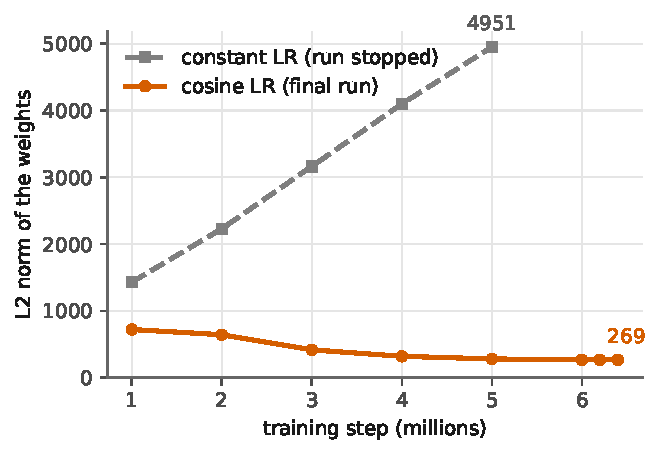
\includegraphics[width=0.85\columnwidth]{fig_weight_norm.pdf}
  \caption{Overall $L_2$ norm of the UNet-B weights along training, from the checkpoints of the two bf16 runs on the same cloud GPU, both with weight decay and gradient clipping: constant learning rate (stopped) against cosine schedule (final run).}
  \label{fig:weight-norm}
\end{figure}

\section{Registered Controls and Pre-Launch Amendments}\label{app:controls}

The sensitivity of co-primary B to the exclusion floor and to the DiT boundary, and the per-layer profiles behind Figure~\ref{fig:localization}, are reported in Section~\ref{sec:confirmatory}; the full per-layer values and the detector AUC at every budget, with their confidence intervals, are in the analysis artifacts of the repository. The matched-quality control was selected by a registered rule: the DiT checkpoint whose 50\,000-sample FID is closest to the UNet's 99.14 within $[80, 110]$. A pre-check on same-regime checkpoints of the final run at 4M and 5M steps gave 5000-sample FIDs of 77.7 and 75.8, too close to the final DiT, so the batch-64 run stopped at 150\,000 steps was used, with the regime difference declared. The control leg was run at the primary budget only, with 500 seeds.

Two implementation amendments were registered before launch, when no confirmatory data existed, to cut a forecast of about 57 hours of wall-clock time, two thirds of it in singular-value decompositions on sampler steps that no registered test consumes. Singular values are obtained from the eigenvalues of $A^\top A$, 1.9 times faster, with a measured deviation from the direct decomposition of at most $7.6{\times}10^{-4}$ per cell and at most $4.4{\times}10^{-6}$ on the input of co-primary A against its margin of 0.010 (every registered statistic moves at least 300 times less than its threshold), guarded at runtime by a recomputation that aborts above $2{\times}10^{-3}$ per cell; in the 50- and 100-step transfer runs the hooks fire only on the late window, which leaves the registered statistics bit-identical. The forecast fell to about 28 hours and the grid ran in 25 hours and 47 minutes.

\section{Reproducibility}\label{app:repro}

\textbf{Seeds.} The sampler is deterministic given $(z_T, y)$. The pilot used base seed 20260705 with labels $y_i = 10 i \bmod 1000$ over 100 seeds; the confirmatory study used base seed 21260705, disjoint by construction, with $z_T$ of sample $i$ drawn from seed $\mathrm{BASE} + i$ and labels 0 to 499, shared across models and budgets. The Rademacher branch is drawn from a derived-seed generator. Checkpoints: the DiT and the UNet are the EMA weights of their final runs at step 6\,400\,000; DiT@FID95 is the batch-64 DiT run at step 150\,000.

\textbf{Hardware and software.} One workstation ran everything except the two bf16 UNet runs: Ubuntu 24.04, Intel Core i9-10900K, AMD Radeon RX 6900 XT with 16~GB, ROCm 7.2.2, Python 3.12.3, PyTorch 2.11.0. The bf16 runs used a cloud NVIDIA RTX 3090. Two platform constraints shaped the pipeline: RDNA 2 has no native bf16, so training ran in fp16 or fp32 locally; and batched singular values on ROCm are much slower than on the CPU (a 25-step measurement pass takes 241.8~s on the GPU against 16.2~s on the CPU), so every spectral reduction runs on the CPU.

\textbf{Artifacts.} Every number in this paper is traced to an analysis artifact of the public repository, which also holds the two pre-registrations and the scripts that regenerate every figure. The heavy substrate (checkpoints and per-head metrics for every layer, step and seed, about 700~MB for the confirmatory grid) is not versioned and is available on request.

\end{document}
